% \section{Purpose and Scope}
% % This Software Requirements Specification (SRS) document provides a detailed description of the functionalities, requirements, and architecture for the Route Optimization System. It will serve as a guide for the development team to build the software as per the specified requirements.

% The purpose of this Software Requirements Specification (SRS) document is to outline the software and system requirements for the development of our project Rahguzar, an AI-driven route optimization system. This system aims to address inefficiencies in manual route planning within the retail and distribution sectors, improving operational efficiency and reducing environmental impacts. 

% This document covers both the functional requirements, describing what the system should do, along with the non-functional requirements specifying the system’s performance, scalability, and usability criteria. Moreover, the document includes system block diagrams to visualize system interactions, use cases, and external interfaces, giving a clear and precise idea of the system design and development. 


% \section{Feedback from Presentation}
% % Based on the feedback received during the presentation, additional features like user-friendly mobile compatibility and scalability for larger data volumes were incorporated.
% The feedback received after the proposal presentation to us is summarized below: 

% \begin{itemize}
%     \item \textbf{Expand Literature Review:} Include both AI and non-AI solutions in the literature review to focus on best practices and successful case studies in route optimization. Non-AI methods such as mathematical models and heuristic methods need to be explored.

%     \item \textbf{Clear Parameter Identification:} Clearly define key route optimization parameters, including distance, time windows, traffic, and scalability metrics, for precise algorithm development and performance evaluation.

%     \item \textbf{Gantt Chart Agility: }Suggested discussing potential challenges and making the Gantt chart more agile.

% \end{itemize}


\section{Problem Statement}

% In the vast fields of retail and distribution, route planning for field representatives is often done manually. This leads to multiple inefficiencies such as increased travel times, missed sales opportunities, and higher operational costs. Traditional manual route planning can be ineffective as it does not account for multiple critical variables such as traffic patterns, store service hours, and location-based priorities. This results in suboptimal routes that require more fuel consumption and increased travel costs. 

% Our proposed solution, Rahguzar, aims to address these challenges by automating route optimization using advanced algorithms, minimizing travel time, and enhancing productivity. This way, we aim to provide better and optimized routes with the potential for significant time and cost savings and a reduction in carbon footprint.

In the dynamic and ever-evolving world of retail and distribution, planning Permanent Journey Plans (PJP) plays a vital role in organizing daily route schedules for field representatives, such as sales executives, to ensure consistent and efficient service to stores. PJPs involve determining which stores to visit on which days and assigning sales representatives while adhering to predefined constraints such as visit frequencies, even visit spacing, workload balancing, consistent assignments, holidays, and minimizing travel distances.
However, this planning process is inherently complex. Traditional manual or semi-automated approaches are unable to handle the scale and intricacies of modern Fast-Moving Consumer Goods (FMCG) operations, leading to inefficient routes that increase travel times and operational costs. Misaligned schedules result in missed visits or inconsistent service, while poor resource utilization increases inefficiencies. These inefficiencies also contribute to increased fuel consumption and carbon emissions, further escalating costs and environmental impact. Moreover, managing thousands of stores across diverse regions poses significant scalability challenges.

% There is a pressing need for a robust, intelligent system to automate PJP planning and address these challenges by ensuring optimal routes, efficient workforce utilization, and cost-effective operations while reducing the environmental footprint.

To overcome these challenges, Rahguzar is proposed as an innovative web-based solution designed to automate and optimize PJP planning, enabling efficient route generation, effective workforce utilization, and reduced operational and environmental costs.
\section{Proposed Solution}

% The proposed solution, Rahguzar, will be a web-based application that will use an algorithm to optimize routes for field representatives including but not limited to merchandisers, sales representatives, and order bookers. Our algorithm will take variables such as shift times, store profiles, service hours, store priority parameters, and historical traffic data to predict the routes and timings accordingly. This comprehensive approach ensures tailored routes for each representative, maximizing route efficiency and aligning with specific business goals. 

% The solution will provide interactive map interface where managers will have certain features available to them such as visualizing, adjusting, and scheduling visits on a daily, weekly, or monthly basis. The system’s capabilities aim to reduce travel time, operational costs, and environmental impacts.
The proposed solution, Rahguzar, is a comprehensive web-based application developed to automate and optimize the planning of PJPs for distributors, managers, and field representatives, including sales executives, merchandisers, and order bookers, in the FMCG sector. Rahguzar generates efficient, scalable schedules that adhere to critical constraints, such as store visit frequencies, even visit spacing, workload balancing, consistent assignments, holidays, and minimizing travel distances. These tailored schedules ensure that field representatives can execute their tasks effectively while aligning with the organization’s operational goals.

The platform features a user-friendly, interactive map interface that allows managers to visualize, adjust, and schedule visits for daily, weekly, or monthly plans. It provides flexibility for real-time updates, ensuring adaptability to dynamic business needs. Additionally, Rahguzar determines the optimal number of field representatives required, improving workforce utilization and preventing inefficiencies such as overstaffing or under-hiring.

By optimizing routes, Rahguzar minimizes travel times, operational costs, and fuel consumption, significantly reducing the carbon footprint and promoting sustainability. This automation reduces the need for manual intervention, saving valuable time for managers while ensuring that field representatives have clear, efficient routes tailored to their responsibilities. Rahguzar delivers a scalable, cost-effective, and environmentally sustainable solution for modern FMCG operations, enhancing productivity, consistency, and overall service quality.
% This section gives a summary of our proposed solution, i.e. how does it solve the problem? An overview of the system is provided. A detailed description of each module of the system is presented later in Chapter ~\ref{chap:intro}.

\section{Intended User}

This section outlines the target users of Rahguzar, detailing the different types of users in the user base and their interactions with the platform.
\begin{itemize}

         \item \textbf{Managers:} Managers are the primary users of the system, responsible for creating, adjusting, and scheduling optimized journey plans for field representatives. They will interact with the platform through a user-friendly map interface to design, visualize, and modify routes. The system allows managers to generate daily, weekly, or monthly plans, adapt to specific business constraints, and ensure operational efficiency.
         \item \textbf{Field Representatives:} While field representatives, such as sales executives and order bookers, do not directly interact with the system, they are key beneficiaries of its outputs. They rely on the optimized journey plans created by managers to execute their tasks efficiently in the field, ensuring consistent and effective service to stores.
% The primary users of Rahguzar include:

% \begin{itemize}

%     \item \textbf{Managers:} Responsible for creating, adjusting, and scheduling optimized routes for field representatives. They use the system’s map interface to create, visualize and fine-tune routes as needed. They can create these routes based on a daily, weekly, or a monthly basis.

%     % \item \textbf{Field Representatives:} Sales representatives, order bookers, and other field staff who receive pre-defined routes and visit the set of locations assigned to them.

%     % \item \textbf{Admin/IT Personnel:} Oversee system management, manage user accounts, and ensure data security and system integrity.
    
\end{itemize}


\section{Project Gantt chart and deliverables}

Deliverables for Kaavish I:
\begin{itemize}
    \item Requirements Specification Document
    \item System Architecture \& Design Diagram
    \item Prototype for Frontend and Backend Components
    \item Fully Developed Route Optimization Algorithm
    \item Performance and Evaluation Report
\end{itemize}
Deliverables for Kaavish II:
\begin{itemize}
    \item Comparison with existing Algorithms and improvements
    \item User-friendly web application with map interface
    \item Performance Metrics Dashboard
    \item Pilot Testing Framework and Results
    \item Final Project Documentation and Evaluation Report
\end{itemize}



\begin{center}
        \begin{figure}[H]
        \centering
        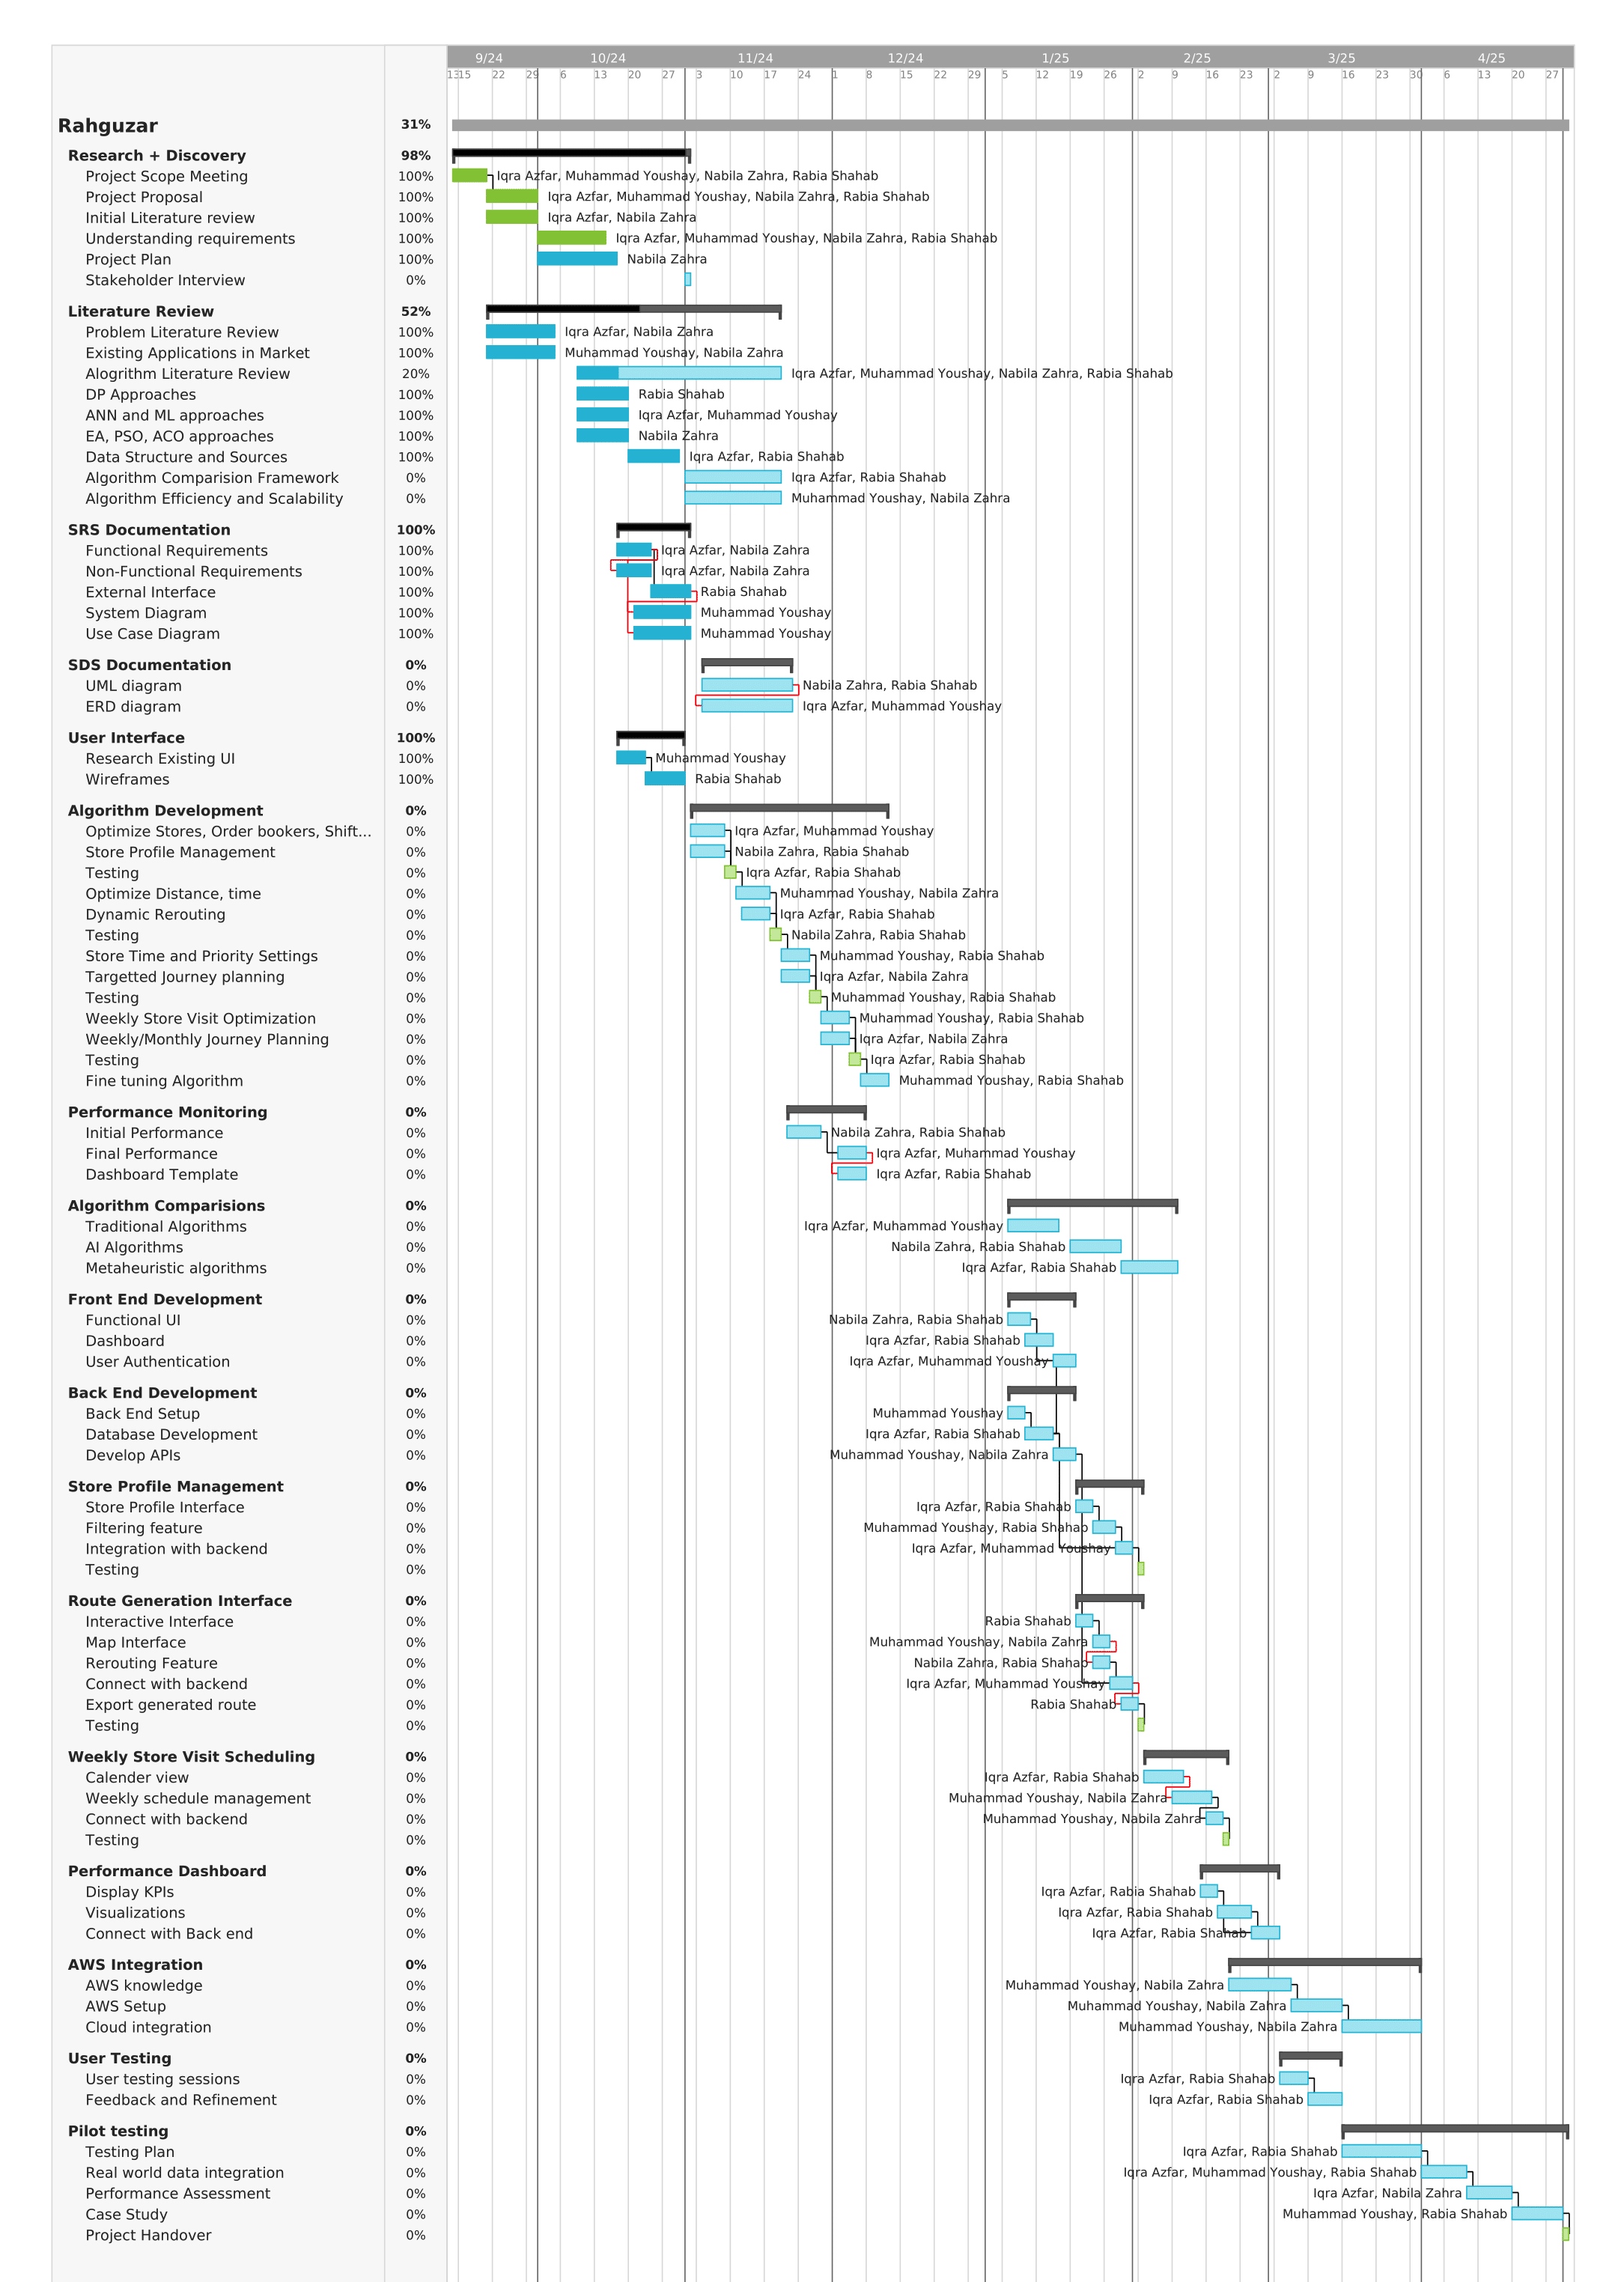
\includegraphics[width=\textwidth]{images/Rahguzar (2)-1.png} 
        \caption{Project Gantt Chart}
    \end{figure}
\end{center}

\section{Key Challenges}

Key challenges anticipated in our project will include:

\begin{itemize}
    \item \textbf{Data Complexity and Integration:} Managing and integrating diverse datasets, including store profiles, geographic data, and workforce schedules, presents significant complexity, particularly in reconciling inconsistencies and ensuring data accuracy. \\
    \textbf{Solution:} Utilize specialized data processing libraries to streamline data handling and incorporate iterative testing phases to identify and address integration issues early in development.

    \item \textbf{Multi-Objective Optimization:} Balancing multiple optimization criteria, such as minimizing travel distances, reducing costs, meeting visit frequencies, and ensuring workload balancing, is inherently challenging due to competing priorities. \\
    \textbf{Solution:} Implement a weighted scoring system to prioritize objectives based on business needs and evaluate outputs from multiple algorithms to identify the most efficient and effective solutions.

    \item \textbf{API Costs and Performance:} Heavy reliance on mapping APIs, such as Google Maps, could lead to high costs and potentially slow performance when processing large-scale data. \\
    \textbf{Solution:} Optimize API usage through practices like batch processing and caching to reduce the number of API calls. Additionally, utilize trial phases of these services to test and implement them effectively without exceeding cost limits.

    \item \textbf{Adaptability to Business-Specific Constraints:} Organizations may have unique and variable constraints, such as holidays, visit frequency, or workload preferences, which require flexible accommodation in the route planning system. \\
    \textbf{Solution:} Design the system to allow customization of route parameters and enable managers to manually adjust routes through an intuitive interface, ensuring flexibility for diverse business requirements.
  % \item \textbf{Data Complexity and Integration:} Integrating diverse datasets such as store profiles and geographic data, is complex and requires rigorous data reconciliation. \\
    % \textbf{Solution:} Use specialized libraries to streamline data handling and implement iterative testing phases to identify integration issues early.

    % \item \textbf{Multi-Objective Optimization:} Balancing multiple route optimization criteria (time, cost, distance, etc.) is challenging. \\
    % \textbf{Solution:} Apply a weighted scoring system to prioritize objectives and compare outputs from different algorithms to determine efficiency among them.

    % \item \textbf{API Costs and Performance:} Heavy reliance on Google Maps API may incur costs and slow performance. \\
    % \textbf{Solution:} Implement efficient API usage practices, such as batch processing, to minimize calls and costs. Moreover, we aim to utilize the trial phases of these services to implement them in our project. 

    % \item \textbf{Adaptability for Business-Specific Constraints:} Organizations may have unique, varying constraints that the model needs to accommodate flexibly. \\
    % \textbf{Solution:} Allow customization of route parameters and provide managers with control to manually adjust routes based on specific business needs.
    
\end{itemize}